\chapter{Arhitektura i dizajn sustava}
	
	Za ostvarenje naše aplikacije odabrali smo arhitekturu zasnovanu na događajima. Prednosti ovog tipa arhitekture su mnoge: 
	\begin{itemize}
		\item svaki od servisa arhitekture može biti neovisan entitet, što povećava fleksibilnost 
		\item događaji se mogu pratiti u stvarnom vremenu, što olakšava analizu sustava
		\item događaji predstavljaju promjene stanja pa je komponentama omogućeno da reagiraju na te promjene
	\end{itemize}
	
				\begin{figure}[H]
			\includegraphics[scale=0.4]{slike/event\_driven\_architecture.PNG} %veličina slike u odnosu na originalnu datoteku i pozicija slike
			\centering
			\caption{Prikaz arhitekture zasnovane na događajima}
			\label{event_driven_architecture}
		\end{figure}
		
	Specifično, radi se o MVC (Model-View-Controller) obrascu, koji odvaja korisničko sučelje od ostatka sustava. On dodatno smanjuje međuovisnost U/I sučelja i ostatka sustava. Sastoji se od tri dijela:
	
		\begin{itemize}
			\item model - sadrži razrede čiji se objekti obrađuju različitim operacijama. Odgovoran je za održavanje dosljednosti podataka te obavljanje poslovnih operacija i pravila
			\item view (pogled) - odgovoran za prezentaciju podataka korisnicima (korisničko sučelje, web-aplikacija, grafovi...). On ne bi trebao sadržavati nikakvu poslovnu logiku, već prikazuje informacije korisnicima na razunmljiv i privlačan način
			\item controller (nadglednik) - sadrži razrede koji upravljaju i rukuju korisničkom interakcijom s pogledom i modelom
		\end{itemize}
		
			\begin{figure}[H]
			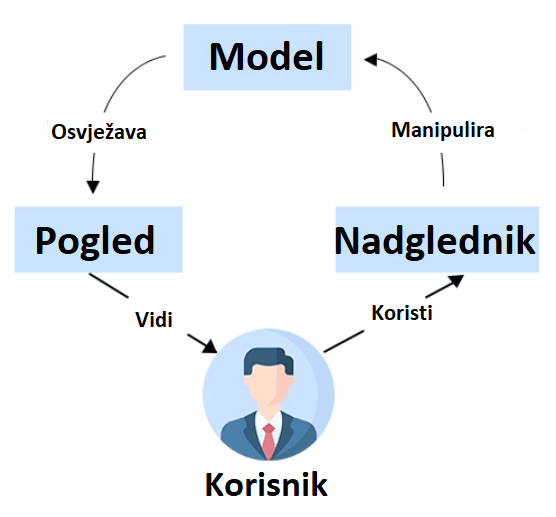
\includegraphics[scale=0.4]{slike/mvc.PNG} %veličina slike u odnosu na originalnu datoteku i pozicija slike
			\centering
			\caption{Prikaz načina rada MVC obrasca}
			\label{mvc}
		\end{figure}
		
	Po principu oblikovanja arhitekture odabrali smo \textit{Podijeli pa vladaj} arhitekturu, kako bismo se unutar tima mogli podijeliti u manje timove koji rade na određenim problemima i kako bismo, ako to bude bilo potrebno, jednostavno zamijenili željene dijelove bez opsežne intervencije u cijeli sustav.
	
			\begin{figure}[H]
			\includegraphics[scale=0.4]{slike/divide\_and\_conquer.PNG} %veličina slike u odnosu na originalnu datoteku i pozicija slike
			\centering
			\caption{Prikaz principa djelovanja "podijeli pa vladaj"}
			\label{divide_and_conquer}
		\end{figure}
		
	Arhitektura našeg sustava dijeli se na tri komponente:
	\begin{itemize}
		\item Web preglednik - softverska aplikacija koja omogućuje korisnicima pregledavanje i interakciju sa svim sadržajima Interneta. Glavna funkcija web preglednika je prikazivanje web stranica koje su oblikovane u obliku programskog koda na korisniku jasan način. Neki poznati web-preglednici uključuju Google Chrome, Mozilla Firefox, Opera...Web preglednik služi i kao medijator između korisnika, koji šalje zahtjeve, i web poslužitelja, koji prima zahtjeve i na njih odgovara.
		\item Web poslužitelj - program koji prosljeđuje web sadržaje web klijentu/pregledniku na njegov zahtjev putem protokola HTTP. On od klijenta dobije zahtjev za podacima, pristupa bazi podataka (kojoj također ima pristup), dohvaća tražene podatke iz baze te ih vraća klijentu u obliku HTTP odgovora. Vraćeni podaci se zatim prikazuju klijentu (ako nije došlo do poteškoća).
		\item Baza podataka - omogućuje organiziranu pohranu podataka koje je potrebno pohraniti (za KuhajIT su to podaci o korisničkim profilima, recepti, kuharice, osvrti na recepte, proizvodi i ostali)
	\end{itemize}
	
		\begin{figure}[H]
			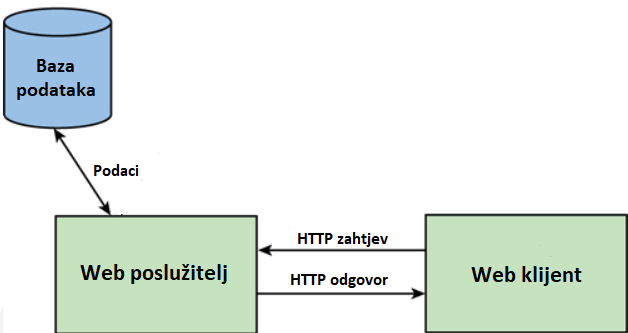
\includegraphics[scale=0.4]{slike/architecture.PNG} %veličina slike u odnosu na originalnu datoteku i pozicija slike
			\centering
			\caption{Prikaz principa djelovanja podsustava arhitekture}
			\label{architecture}
		\end{figure}
	

	Čitavi backend naše aplikacije izrađen je u programskom jeziku \textit{Java}, u radnom okviru \textit{Spring Boot}. Razvojno okruženje korišteno za razvoj backenda je \textit{Eclipse IDE}.
	Frontend je izrađen u programskom jeziku \textit{JavaScript}, u biblioteci \textit{React}. Razvojno okruženje korišteno za razvoj frontenda je \textit{Visual Studio Code}.
			
		\section{Baza podataka}

		Za ostvarenje naše aplikacije KuhajIT odabrali smo relacijsku bazu podataka PostgreSQL, u alatu \textit{PGadmin4}, koja svojom jednostavnom i lako razumljivom strukturom olakšava pregled i upravljanje podacima. Ključne komponente relacijske baze podataka su entiteti (tablice okarakterizirane imenom i skupom atributa) te veze među entitetima (strukture koje povezuju podatke iz različitih entiteta pomoću ključeva).
		
		Entiteti naše baze podataka su:
		\begin{itemize}
			\item User
			\item Role
			\item Recipe
			\item Recipe Ingredient
			\item Ingredient
			\item Cookbook
			\item Cookbook Recipe
			\item Review
			\item Response
			\item Image
			\item Recipe Image
			\item Diet
			\item Diet Ingredient
			\item Diet allowed recipes
			\item Consumed recipes
			\item Step of making
			\item Category
			\item Label
		\end{itemize}
		
		
			\subsection{Opis tablica}
				
				\textbf{User} Entitet \textit{User} sadrži atribute važne za svakog registriranog korisnika aplikacije KuhajIT. Ti atributi su: ID korisnika, korisničko ime, lozinku, ime, prezime, email, uloga, biografija, ID osobne fotografije koju je priložio, oznaka potvrđenosti i ID dijete koje se pridržava. U vezi je \textit{One-to-Many} s entitetom \textit{Review} preko korisničkog ID-ja, \textit{One-to-Many} s entitetom \textit{Cookbook} preko korisničkog ID-ja, \textit{Recipe} preko korisničkog ID-ja, \textit{One-to-Many} s entitetom \textit{Response} preko korisničkog ID-ja, \textit{One-to-One} s entitetom \textit{Image} preko ID-ja učitane fotografije, \textit{Many-to-One} s entitetom \textit{Role} preko ID-ja uloge, \textit{Many-to-One} s entitetom \textit{Diet} preko ID-ja dijete i \textit{One-to-Many} s entitetom \textit{Consumed Recipes} preko ID-ja korisnika.
				
				\begin{longtblr}[
					label=none,
					entry=none
					]{
						width = \textwidth,
						colspec={|X[8,l]|X[6, l]|X[20, l]|}, 
						rowhead = 1,
					} %definicija širine tablice, širine stupaca, poravnanje i broja redaka naslova tablice
					\hline \SetCell[c=3]{c}{\textbf{User}}	 \\ \hline[3pt]
					\SetCell{LightGreen}id & INT	&  	ID korisnika, sekvencijski generiran.  	\\ \hline
					username 	& VARCHAR &  Korisničko ime korisnika, koje mora biti jedinstveno, korisnik si ga bira sam pri registraciji, no može ga promijeniti. 	\\ \hline 
					password & VARCHAR & Lozinka za pristup korisničkom računu. \\ \hline
					name & VARCHAR	&  	Ime korisnika	\\ \hline 
					surname & VARCHAR & Prezime korisnika \\ \hline
					email & VARCHAR &   Ako se korisnik želi registrirati kao kulinarski entuzijast/nutricionist, mora priložiti email, inače atribut poprima NULL vrijednost.\\ \hline 
					confirmed & BOOLEAN & Oznaka je li administrator potvrdio registraciju kulinarskog entuzijasta/nutricionista.\\ \hline	
					biography & VARCHAR & Ako se korisnik želi registrirati kao kulinarski entuzijast/nutricionist, mora priložiti kratku biografiju, inače atribut poprima NULL vrijednost.\\ \hline
			\SetCell{LightBlue}image\_id & INT & ID osobne fotografije koju je korisnik koji želi biti kulinarski entuzijast ili nutricionist učitao. \\ \hline
			\SetCell{LightBlue}role\_id	& INT &   ID uloge koju korisnik registracijom želi posjedovati (nutricionist, kulinarski entuzijast ili klijent).\\ \hline
			\SetCell{LightBlue}diet\_id	& INT &   ID dijete koje se korisnik pridržava.	\\ \hline
				\end{longtblr}
				
				\textbf{Role} Entitet \textit{Role} je šifarnik uloga koje korisnik registracijom može dobiti. To su:
				\begin{itemize}
					\item klijent
					\item nutricionist
					\item kulinarski entuzijast
				\end{itemize}
				
				Uz navedene, u tablici se nalazi i uloga administratora, koju nije moguće dobiti registracijom u sustav, već je predefiniran. U vezi je \textit{One-to-Many} s entitetom \textit{User}, preko ID-ja uloge.
				
				\begin{longtblr}[
					label=none,
					entry=none
					]{
						width = \textwidth,
						colspec={|X[8,l]|X[6, l]|X[20, l]|}, 
						rowhead = 1,
					} %definicija širine tablice, širine stupaca, poravnanje i broja redaka naslova tablice
					\hline \SetCell[c=3]{c}{\textbf{Role}}	 \\ \hline[3pt]
					\SetCell{LightGreen}id & INT	&  Jedinstveni	ID uloge, sekvencijski generiran.  	\\ \hline
					name & VARCHAR	&  Naziv uloge.	\\ \hline 
				\end{longtblr}
				
				\textbf{Recipe} Entitet \textit{Recipe} sadrži atribute važne za svaki recept objavljen na web aplikaciji KuhajIT. Ti atributi su: ID recepta, ime recepta, vrijeme pripreme, ID autora recepta, veličina porcije, ID kategorije kojoj pripada recept. U vezi je \textit{One-to-Many} s entitetom \textit{Recipe Image} preko ID-ja recepta, \textit{One-to-Many} s entitetom \textit{Cookbook Recipe} preko ID-ja recepta, \textit{One-to-Many} s entitetom \textit{Recipe Ingredient} preko ID-ja recepta, \textit{Many-to-One} s entitetom \textit{User} preko ID-ja korisnika i \textit{Many-to-One} s entitetom \textit{Category}.
				
					\begin{longtblr}[
					label=none,
					entry=none
					]{
						width = \textwidth,
						colspec={|X[8,l]|X[6, l]|X[20, l]|}, 
						rowhead = 1,
					} %definicija širine tablice, širine stupaca, poravnanje i broja redaka naslova tablice
					\hline \SetCell[c=3]{c}{\textbf{Recipe}}	 \\ \hline[3pt]
					\SetCell{LightGreen}id & INT	&  Jedinstveni	ID recepta, sekvencijski generiran.  	\\ \hline
					name & VARCHAR	&  Ime recepta.	\\ \hline
					cook\_time 	& INT &  Vrijeme pripreme recepta. 	\\ \hline 
					portion\_size & INT & Veličina porcije pripremljenog recepta. \\ \hline
					steps\_of\_making & VARCHAR	&  Koraci pripreme recepta.	\\ \hline 
					\SetCell{LightBlue}creator\_id	& INT &   Korisnički ID autora recepta.	\\ \hline 
					\SetCell{LightBlue}category\_id	& INT &   ID kategorije kojoj recept pripada.	\\ \hline 
				\end{longtblr}
				
				\textbf{Recipe Ingredient} Entitet \textit{Recipe Ingredient} sadrži atribute važne za pohranu sastojaka koji se koriste u pojedinom receptu objavljenom na web aplikaciji KuhajIT. Ti atributi su: ID sastojka recepta, količina sastojka, ID recepta i ID sastojka. U vezi je \textit{Many-to-One} s entitetom \textit{Recipe} preko ID-ja recepta i \textit{Many-to-One} s entitetom \textit{Ingredient}.
				
				\begin{longtblr}[
					label=none,
					entry=none
					]{
						width = \textwidth,
						colspec={|X[6,l]|X[6, l]|X[20, l]|}, 
						rowhead = 1,
					} %definicija širine tablice, širine stupaca, poravnanje i broja redaka naslova tablice
					\hline \SetCell[c=3]{c}{\textbf{Recipe Ingredient}}	 \\ \hline[3pt]
					\SetCell{LightGreen}ingredient\_id	& INT &   ID sastojka.	\\ \hline
					\SetCell{LightGreen}recipe\_id	& INT & ID recepta. \\ \hline
					quantity & INT &  Količina sastojka potrebnog za recept. 	\\ \hline 
				\end{longtblr}
				
				\textbf{Ingredient} Entitet \textit{Ingredient} sadrži atribute važne za svaki sastojak.
Ti atributi su: ID sastojka i ime sastojka. U vezi je \textit{One-to-Many} s entitetom \textit{Recipe Ingredient} preko ID-ja sastojka, \textit{Many-to-One} s entitetom \textit{Image} preko ID-ja fotografije i \textit{Label} preko ID-ja oznake.

				\begin{longtblr}[
					label=none,
					entry=none
					]{
						width = \textwidth,
						colspec={|X[6,l]|X[6, l]|X[20, l]|}, 
						rowhead = 1,
					} %definicija širine tablice, širine stupaca, poravnanje i broja redaka naslova tablice
					\hline \SetCell[c=3]{c}{\textbf{Ingredient}}	 \\ \hline[3pt]
					\SetCell{LightGreen}id & INT	&  Jedinstveni ID sastojka, sekvencijski generiran.  	\\\hline
					name 	& VARCHAR &  Naziv sastojka. 	\\ \hline 
					\SetCell{LightBlue}image\_id	& INT &   ID fotografije sastojka.	\\ \hline 						\SetCell{LightBlue}label\_id	& INT &   ID oznake sastojka.	\\ \hline 
				\end{longtblr}	
				
				\textbf{Cookbook} Entitet \textit{Cookbook} sadrži atribute važne za svaku kuharicu stvorenu od kulinarskog entuzijasta na web aplikaciji KuhajIT.
Ti atributi su: ID kuharice, ID kategorije kuharice, naziv kuharice i ID autora. U vezi je \textit{One-to-Many} s entitetom \textit{Cookbook Recipe} preko ID-ja kuharice, \textit{Many-to-One} s entitetom \textit{User} preko ID-ja korisnika (kulinarskog entuzijasta koji ju je stvorio) i \textit{Many-to-One} s entitetom \textit{Category} preko ID-ja kategorije.

				\begin{longtblr}[
					label=none,
					entry=none
					]{
						width = \textwidth,
						colspec={|X[6,l]|X[6, l]|X[20, l]|}, 
						rowhead = 1,
					} %definicija širine tablice, širine stupaca, poravnanje i broja redaka naslova tablice
					\hline \SetCell[c=3]{c}{\textbf{Cookbook}}	 \\ \hline[3pt]
					\SetCell{LightGreen}id & INT	&  Jedinstveni ID kuharice, sekvencijski generiran.  	\\ \hline
					category 	& VARCHAR &  Kategorija kuharice. 	\\ \hline 
					name & VARCHAR & Naziv kuharice. \\ \hline
					\SetCell{LightBlue}creator\_id	& INT &   Korisnički ID autora kuharice.	\\ \hline 
					\SetCell{LightBlue}category\_id	& INT &  ID kategorije kuharice.	\\ \hline 
					
				\end{longtblr}
				
		\textbf{Cookbook Recipe} Entitet \textit{Cookbook Recipe} sadrži atribute važne za pohranu recepata u pojedinu kuharicu na web aplikaciji KuhajIT.
Ti atributi su: ID kuharice i ID recepta. U vezi je \textit{Many-to-One} s entitetom \textit{Cookbook} preko ID-ja kuharice i \textit{Many-to-One} s entitetom \textit{Recipe} preko ID-ja recepta koji se u kuharici nalazi.

			\begin{longtblr}[
					label=none,
					entry=none
					]{
						width = \textwidth,
						colspec={|X[6,l]|X[6, l]|X[20, l]|}, 
						rowhead = 1,
					} %definicija širine tablice, širine stupaca, poravnanje i broja redaka naslova tablice
					\hline \SetCell[c=3]{c}{\textbf{Cookbook Recipe}}	 \\ \hline[3pt]
					\SetCell{LightGreen}cookbook\_id & INT	&  ID kuharice.  	\\ \hline
					\SetCell{LightGreen}recipe\_id 	& INT &  ID recepta. 	\\ \hline				
				\end{longtblr}
				
				\textbf{Review} Entitet \textit{Review} sadrži atribute važne za svaku recenziju ostavljenu na recept na web aplikaciji KuhajIT.
Ti atributi su: ID recenzije, ocjena recepta dodijeljena u recenziji, poruka ostavljena u recenziji, ID autora recenzije i ID recepta na koji je recenzija ostavljena. U vezi je \textit{One-to-Many} s entitetom \textit{Cookbook Recipe} preko ID-ja kuharice i \textit{Many-to-One} s entitetom \textit{User} preko ID-ja korisnika koji je ostavio recenziju, \textit{Many-to-One} s entitetom \textit{Recipe} preko ID-ja recepta na koji je recenzija ostavljena i \textit{One-to-One} s entitetom \textit{Response} preko ID-ja recenzije.

\begin{longtblr}[
					label=none,
					entry=none
					]{
						width = \textwidth,
						colspec={|X[6,l]|X[6, l]|X[20, l]|}, 
						rowhead = 1,
					} %definicija širine tablice, širine stupaca, poravnanje i broja redaka naslova tablice
					\hline \SetCell[c=3]{c}{\textbf{Review}}	 \\ \hline[3pt]
					\SetCell{LightGreen}id & INT	&  Jedinstveni ID recenzije, sekvencijski generiran.  	\\ \hline
					mark 	& INT &  Ocjena ostavljena u recenziji. 	\\ \hline 
					message & VARCHAR & Poruka ostavljena u recenziji. \\ \hline
					\SetCell{LightBlue}creator\_id & INT &   Korisnički ID autora recenzije, ako je recenziju ostavio neregistrirani korisnik, poprima vrijednost NULL.	\\ \hline 
					\SetCell{LightBlue} recipe\_id & INT &   ID recepta na kojeg je recenzija ostavljena.	\\ \hline 
					\SetCell{LightBlue} response\_id & INT &   ID odgovora na recenziju.	\\ \hline 
					\end{longtblr}


\textbf{Response} Entitet \textit{Response} sadrži atribute važne za svaki odgovor na recenziju ostavljenu na recept na web aplikaciji KuhajIT.
Ti atributi su: ID odgovora, poruka ostavljena u odgovoru, ID autora odgovora (kulinarski entuzijast na čiji je recept ostavljena recenzija) i ID recenzije na koju je odgovor ostavljen. U vezi je \textit{One-to-One} s entitetom \textit{Review} preko ID-ja recenzije i \textit{Many-to-One} s entitetom \textit{User} preko ID-ja korisnika koji odgovara na recenziju.
				
			\begin{longtblr}[
					label=none,
					entry=none
					]{
						width = \textwidth,
						colspec={|X[6,l]|X[6, l]|X[20, l]|}, 
						rowhead = 1,
					} %definicija širine tablice, širine stupaca, poravnanje i broja redaka naslova tablice
					\hline \SetCell[c=3]{c}{\textbf{Response}}	 \\ \hline[3pt]
					\SetCell{LightGreen}id & INT	&  Jedinstveni ID odgovora na recenziju, sekvencijski generiran.\\\\ \hline
					message & VARCHAR & Poruka ostavljena u odgovoru na recenziju. \\ \hline
					\SetCell{LightBlue}creator\_id	& INT &   Korisnički ID autora odgovora na recenziju.	\\ \hline 
					\SetCell{LightBlue}review\_id & INT &   ID recenzije na koju autor recepta odgovara.	\\ \hline 
					
				\end{longtblr}
				
				\textbf{Image} Entitet \textit{Image} sadrži atribute važne za svaku fotografiju učitanu u sklopu recepta na web aplikaciji KuhajIT.
Ti atributi su: ID fotografije i URL fotografije.

				\begin{longtblr}[
					label=none,
					entry=none
					]{
						width = \textwidth,
						colspec={|X[6,l]|X[6, l]|X[20, l]|}, 
						rowhead = 1,
					} %definicija širine tablice, širine stupaca, poravnanje i broja redaka naslova tablice
					\hline \SetCell[c=3]{c}{\textbf{Image}}	 \\ \hline[3pt]
					\SetCell{LightGreen}id & INT	&  Jedinstveni ID učitane fotografije, sekvencijski generiran. \\ \hline
					url & VARCHAR & URL učitane fotografije. \\ \hline	
					description & VARCHAR & Opis učitane fotografije. \\ \hline
				\end{longtblr}
				
				\textbf{Recipe Image} Entitet \textit{Recipe Image} sadrži referencu na slike koje je kulinarski entuzijast učitao pri stvaranju recepta. U vezi je \textit{One-to-One} s entitetom \textit{Image} i \textit{Many-to-One} s entitetom \textit{Recipe}.
				
				\begin{longtblr}[
					label=none,
					entry=none
					]{
						width = \textwidth,
						colspec={|X[6,l]|X[6, l]|X[20, l]|}, 
						rowhead = 1,
					} %definicija širine tablice, širine stupaca, poravnanje i broja redaka naslova tablice
					\hline \SetCell[c=3]{c}{\textbf{Recipe Image}}	 \\ \hline[3pt]
					\SetCell{LightGreen}image\_id & INT	&  ID učitane fotografije.  	\\ \hline
					\SetCell{LightBlue}recipe\_id & INT & ID recepta kojem učitana fotografija pripada. \\ \hline	
				\end{longtblr}
				
				\textbf{Diet} Entitet \textit{Diet} sadrži atribute važne za svaku dijetu koju kreira nutricionist. Ti atributi su: ID dijete, naziv dijete, opis dijete i ID nutricionista koji ju je stvorio. U vezi je \textit{Many-to-One} s entitetom \textit{User} preko ID-ja korisnika i \textit{One-to-Many} s entitetom \textit{Diet Ingredient} preko ID-ja dijete..
				
				\begin{longtblr}[
					label=none,
					entry=none
					]{
						width = \textwidth,
						colspec={|X[6,l]|X[6, l]|X[20, l]|}, 
						rowhead = 1,
					} %definicija širine tablice, širine stupaca, poravnanje i broja redaka naslova tablice
					\hline \SetCell[c=3]{c}{\textbf{Diet}}	 \\ \hline[3pt]
					\SetCell{LightGreen}id & INT	&  ID stvorene dijete.  	\\ \hline
					name & VARCHAR &  Naziv dijete. 	\\ \hline 
					description & VARCHAR &  Opis dijete. 	\\ \hline 
					\SetCell{LightBlue}creator\_id & INT & ID nutricionista koji je stvorio dijetu. \\ \hline	
				\end{longtblr}
				
				\textbf{Diet Ingredient} Entitet \textit{Diet Ingredient} sadrži atribute važne za pohranu sastojaka koji su dozvoljeni i preporučeni za konzumiranje u pojedinoj dijete objavljenoj na web-aplikaciji KuhajIT. Ti atributi su: ID dijete, ID sastojka i maksimalna dopuštena gramaža sastojka. U vezi je \textit{Many-to-One} s entitetom Diet preko ID-ja dijete i \textit{Many-to-One} s entitetom Ingredient preko ID-ja sastojka.
				
				\begin{longtblr}[
					label=none,
					entry=none
					]{
						width = \textwidth,
						colspec={|X[9,l]|X[6, l]|X[17, l]|}, 
						rowhead = 1,
					} %definicija širine tablice, širine stupaca, poravnanje i broja redaka naslova tablice
					\hline \SetCell[c=3]{c}{\textbf{Diet Ingredient}}	 \\ \hline[3pt]
					\SetCell{LightGreen}diet\_id & INT	&  ID dijete.  	\\ \hline
					\SetCell{LightGreen}ingredient\_id & INT	&  ID sastojka.  	\\ \hline
					max\_amount\_grams & INT &  Maksimalna dopuštena gramaža . 	\\ \hline 
				\end{longtblr}
				
				\textbf{Diet allowed recipes} Entitet \textit{Diet allowed recipes} sadrži atribute važne za pohranu recepata koji su dozvoljeni za konzumiranje u pojedinoj dijeti objavljenoj na KuhajIT web-aplikaciji. Ti atributi su: ID recepta i ID dijete. U vezi je \textit{Many-to-One} s entitetom \textit{Diet} preko ID-ja dijete i \textit{Many-to-One} s entitetom \textit{Recipe}.
				
				\begin{longtblr}[
					label=none,
					entry=none
					]{
						width = \textwidth,
						colspec={|X[9,l]|X[6, l]|X[17, l]|}, 
						rowhead = 1,
					} %definicija širine tablice, širine stupaca, poravnanje i broja redaka naslova tablice
					\hline \SetCell[c=3]{c}{\textbf{Diet allowed recipes}}	 \\ \hline[3pt]
					\SetCell{LightGreen}diet\_id & INT	&  ID dijete.  	\\ \hline
					\SetCell{LightGreen}recipe\_id & INT	&  ID recepta.  	\\ \hline
				\end{longtblr}
				
				\textbf{Consumed recipes} Entitet \textit{Consumed recipes} sadrži atribute važne za pohranu recepata konzumiranih od registriranog korisnika. Ti atributi su: ID recepta koji je konzumiran, ID korisnika koji ga je konzumirao te datum konzumiranja. U vezi je \textit{Many-to-One} s entitetom \textit{Recipe} preko ID-ja recepta te \textit{Many-to-One} s entitetom \textit{User} preko ID-ja korisnika.
				\begin{longtblr}[
					label=none,
					entry=none
					]{
						width = \textwidth,
						colspec={|X[9,l]|X[6, l]|X[17, l]|}, 
						rowhead = 1,
					} %definicija širine tablice, širine stupaca, poravnanje i broja redaka naslova tablice
					\hline \SetCell[c=3]{c}{\textbf{Consumed recipes}}	 \\ \hline[3pt]
					\SetCell{LightGreen}recipe\_id & INT	&  ID recepta.  	\\ \hline
					\SetCell{LightGreen}user\_id & INT	&  ID korisnika.  	\\ \hline
					date & DATE & Datum unosa. \\ \hline
				\end{longtblr}
				
				\textbf{Step of making} Entitet \textit{Step of making} sadrži atribute važne za korak priprave recepta. Ti atributi su: ID koraka, tekstualni opis koraka, redni broj koraka, ID fotografije koja odgovara tom koraku i ID recepta na koji se korak odnosi. U vezi je \textit{Many-to-One} s entitetom \textit{Recipe} preko ID-ja recepta i \textit{Many-to-One} s entitetom \textit{Image} preko ID-ja fotografije.
				
				\begin{longtblr}[
					label=none,
					entry=none
					]{
						width = \textwidth,
						colspec={|X[9,l]|X[6, l]|X[17, l]|}, 
						rowhead = 1,
					} %definicija širine tablice, širine stupaca, poravnanje i broja redaka naslova tablice
					\hline \SetCell[c=3]{c}{\textbf{Step of making}}	 \\ \hline[3pt]
					\SetCell{LightGreen}id & INT	&  ID koraka izrade.  	\\ \hline
					\SetCell{LightGreen}description & VARCHAR	&  Tekstualni opis koraka.  	\\ \hline
					step\_num & INT & Redni broj koraka. \\ \hline
					\SetCell{LightBlue}image\_id & INT & ID fotografije koraka. \\ \hline
					\SetCell{LightBlue}recipe\_id & INT & ID recepta na koji se korak odnosi. \\ \hline
				\end{longtblr}
				
				\textbf{Category} Entitet \textit{Category} sadrži atribute važne za pohranu kategorija recepata i kuharica. Ti atributi su: ID kategorije i naziv kategorije. U vezi je \textit{One-to-Many} s entitetom \textit{Recipe} preko ID-ja kuharice i \textit{One-to-Many} s entitetom Cookbook preko ID-ja kuharice.
				
								\begin{longtblr}[
					label=none,
					entry=none
					]{
						width = \textwidth,
						colspec={|X[9,l]|X[6, l]|X[17, l]|}, 
						rowhead = 1,
					} %definicija širine tablice, širine stupaca, poravnanje i broja redaka naslova tablice
					\hline \SetCell[c=3]{c}{\textbf{Category}}	 \\ \hline[3pt]
					\SetCell{LightGreen}id & INT	&  ID kategorije.  	\\ \hline
					
					name & VARCHAR & Naziv kategorije. \\ \hline
				\end{longtblr}
				
				
				\textbf{Label} Entitet \textit{Label} sadrži atribute važne za pohranu oznaka proizvoda koje unosi nutricionist. Ti atributi su: ID oznake i naziv oznake. U vezi je \textit{One-to-Many} s entitetom \textit{Ingredient} preko ID-ja oznake.
				
								\begin{longtblr}[
					label=none,
					entry=none
					]{
						width = \textwidth,
						colspec={|X[9,l]|X[6, l]|X[17, l]|}, 
						rowhead = 1,
					} %definicija širine tablice, širine stupaca, poravnanje i broja redaka naslova tablice
					\hline \SetCell[c=3]{c}{\textbf{Label}}	 \\ \hline[3pt]
					\SetCell{LightGreen}id & INT	&  ID oznake.  	\\ \hline
					
					name & VARCHAR & Naziv oznake. \\ \hline
				\end{longtblr}
				
				
				
				
				
				
				
				
				
				
			\begin{figure}[H]
			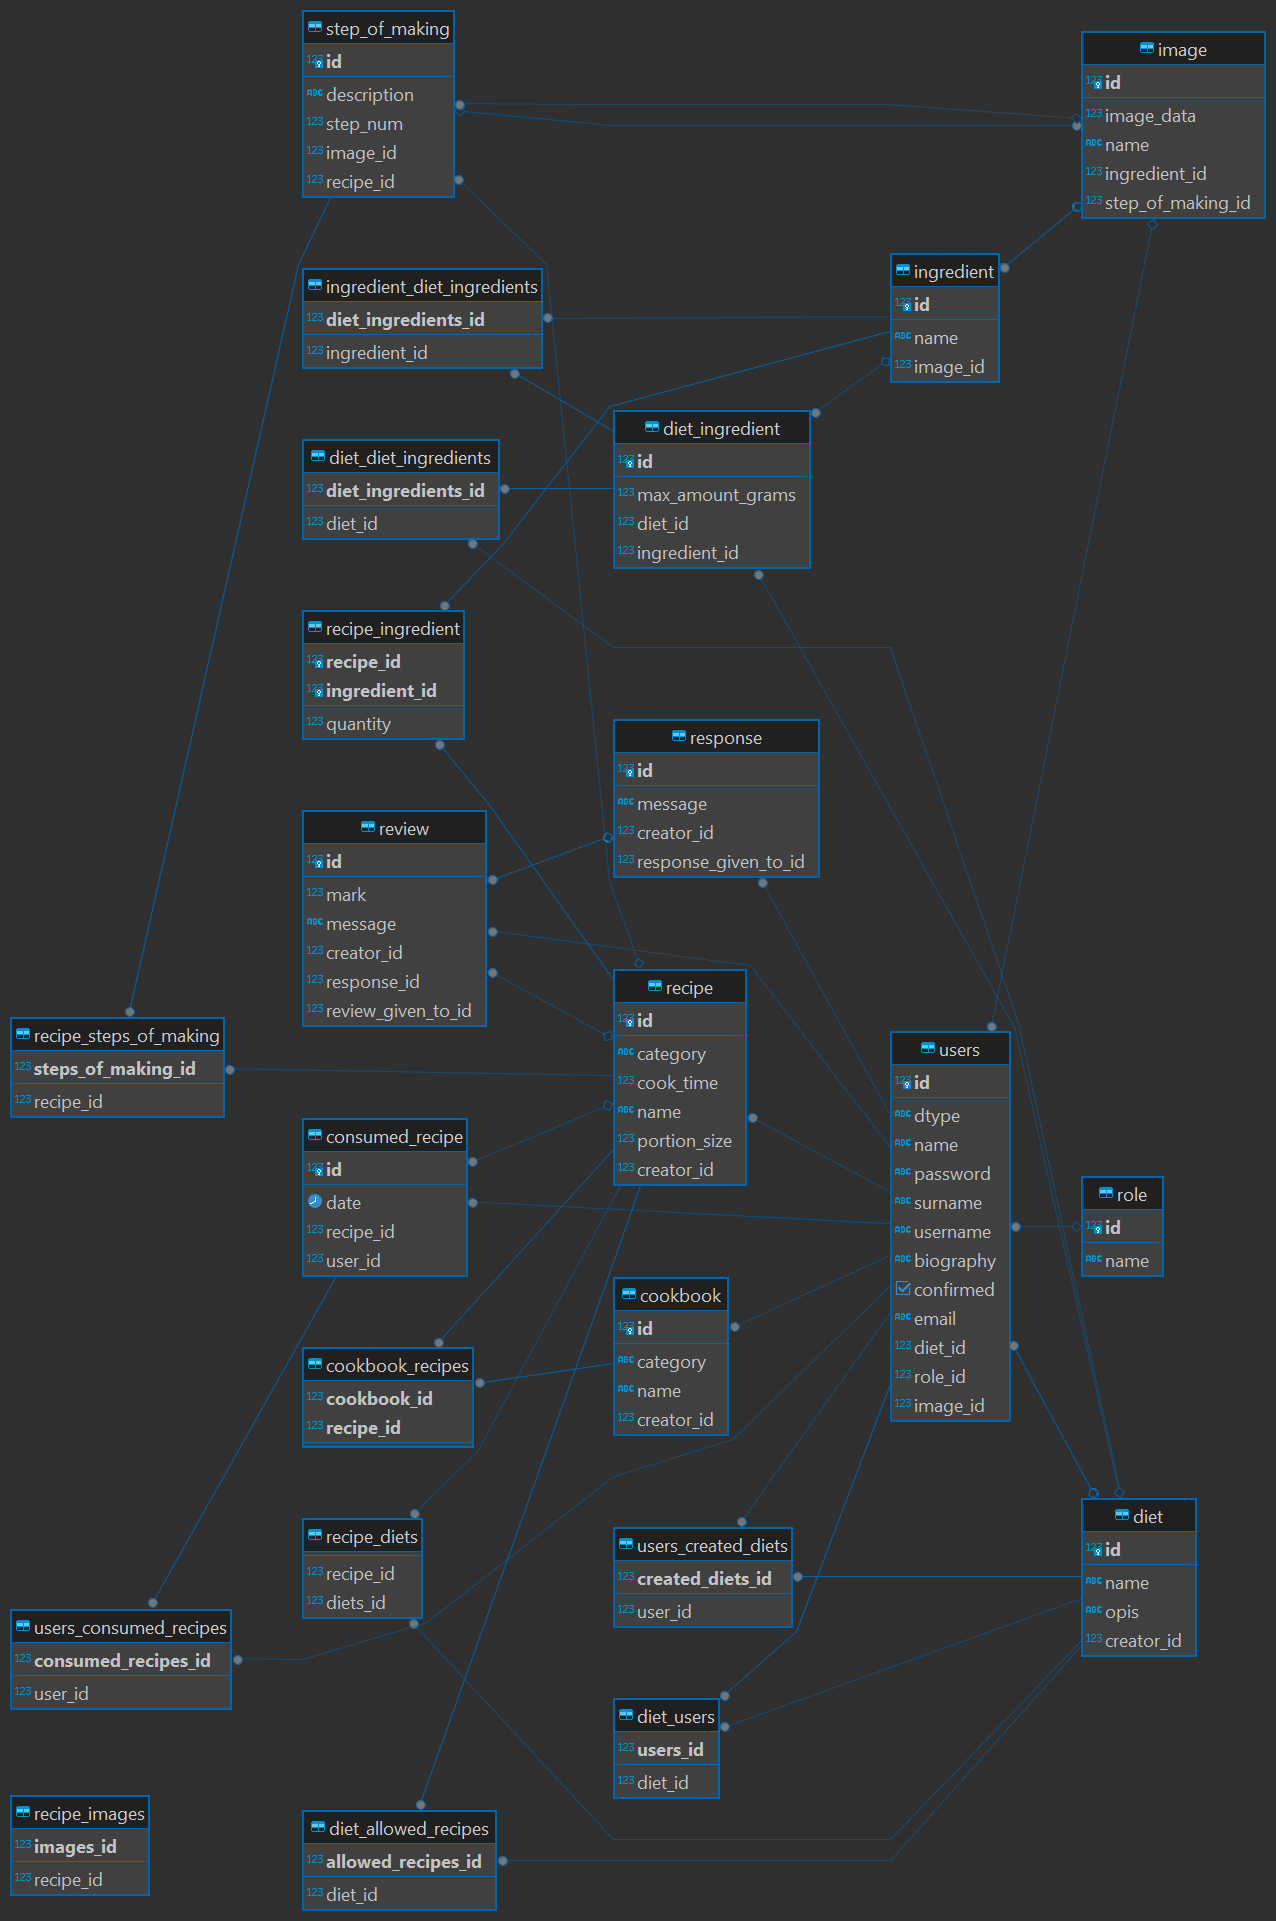
\includegraphics[scale=0.3]{slike/er.PNG} %veličina slike u odnosu na originalnu datoteku i pozicija slike
			\centering
			\caption{Prikaz ER dijagrama baze podataka}
			\label{er}
		\end{figure}
				
				\eject	
	
	  \section{Dijagram razreda}
	  
	  Na slikama 4.6, 4.7, 4.8, 4.9 i 4.10 prikazani su dijagrami razreda koji backend arhitekturu ostvarenog sustava. 
	  Dijagram razreda na slici 4.6 prikazuje razred koji nasljeđuje razred \textit{Controller}.  Kontroleri su odgovorni za prihvaćanje zahtjeva od klijenta, izvršavanje određene poslovne logike i generiranje odgovora koji se šalje natrag klijentu. Drugim riječima, kontroleri obrađuju HTTP zahtjeve i odgovaraju na njih.
	  
	  \begin{figure}[H]
			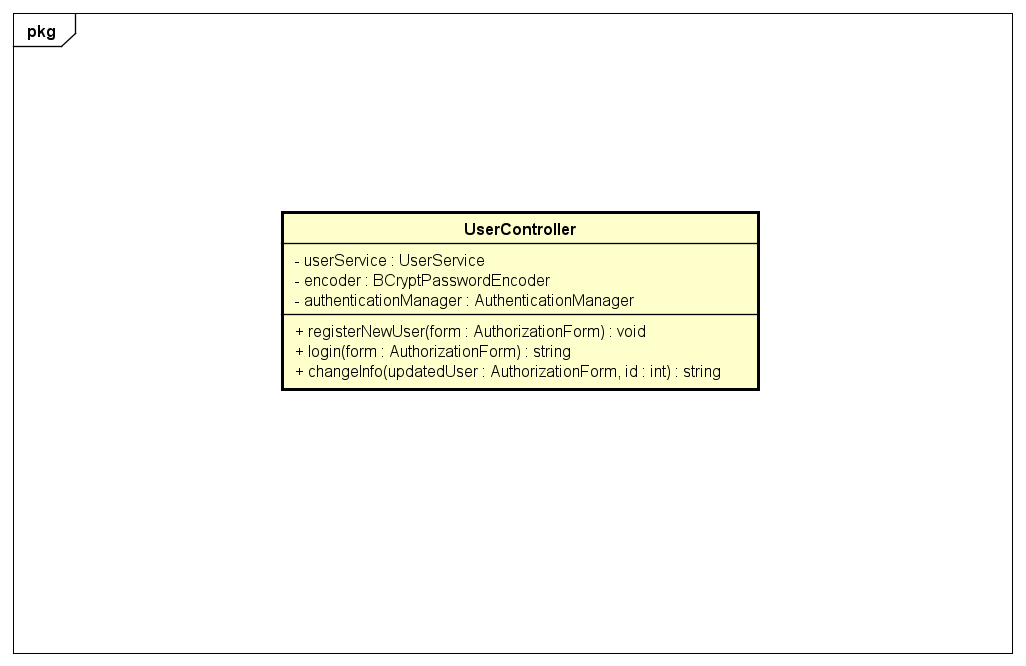
\includegraphics[scale=0.5]{dijagrami/UML_dijagram_razreda_controllers.png} %veličina slike u odnosu na originalnu datoteku i pozicija slike
			\centering
			\caption{Dijagram razreda - dio Controllers}
			\label{Dijagram razreda - dio Controllers}
		\end{figure}
			
			
			\eject 	
			
Dijagram razreda na slici 4.7 prikazuje \textit{Models} dio razreda. \\
	Razredi \textit{Enthusiast} i \textit{Nutritionist} specifikacija su razreda \textit{SpecialUser}, stoga nasljeđuju javne metode i atribute tog razreda, a usto sadrže i metode specifične ulozi. \\
	Razredi \textit{SpecialUser}, \textit{Client} i \textit{Administrator} specifikacija su razreda \textit{User}, stoga nasljeđuju javne metode i atribute tog razreda. \\
	Razred \textit{User} predstavlja korisnika koji se može prijaviti kao klijent, kulinarski entuzijast ili nutricionist te, sukladno svojoj ulozi, obavljati različite funkcije opisane u Specifikaciji programske potpore. \\
    Instanca razreda \textit{User}, ako se radi o registriranom kulinarskom entuzijastu, može stvarati recepte, koji pripadaju razredu \textit{Recipe}, i kuharice, koje pripadaju razredu \textit{Cookbook}. \\
    Razred \textit{Recipe} sadrži sve metode potrebne za stvaranje i objavljivanje recepta. \\
    Razred \textit{Cookbook} sadrži sve metode potrebne za stvaranje tematske kuharice i spremanje recepata u istu. \\
    Razred \textit{Image} sadrži atribute važne za pohranu slika. \\
    Razred \textit{Ingredient} sadrži atribute i metode važne za pohranu i dohvaćanje proizvoda i sastojaka. \\
    Razred \textit{Review} sadrži atribute i metode važne za ostavljanje recenzije na recept kulinarskog entuzijasta. \\
    Razred \textit{Response} sadrži atribute i metode važne za odgovaranje kulinarskog entuzijasta na recenziju ostavljenu na njegov recept.
    Razred \textit{Diet} sadrži atribute i metode važne za stvaranje dijete od nutricionista. 
    Razred \textit{Step of making} sadrži atribute i metode važne za svaki korak izrade recepta od kulinarskog entuzijasta.
    Razredi \textit{Consumed Recipe, Cookbook Recipe, Recipe Ingredient} i \textit{Diet Ingredient} predstavljaju vezne klase između klasa koje povezuju (\textit{Many-to-Many} veze u bazi podataka).
			
			
			\begin{figure}[H]
			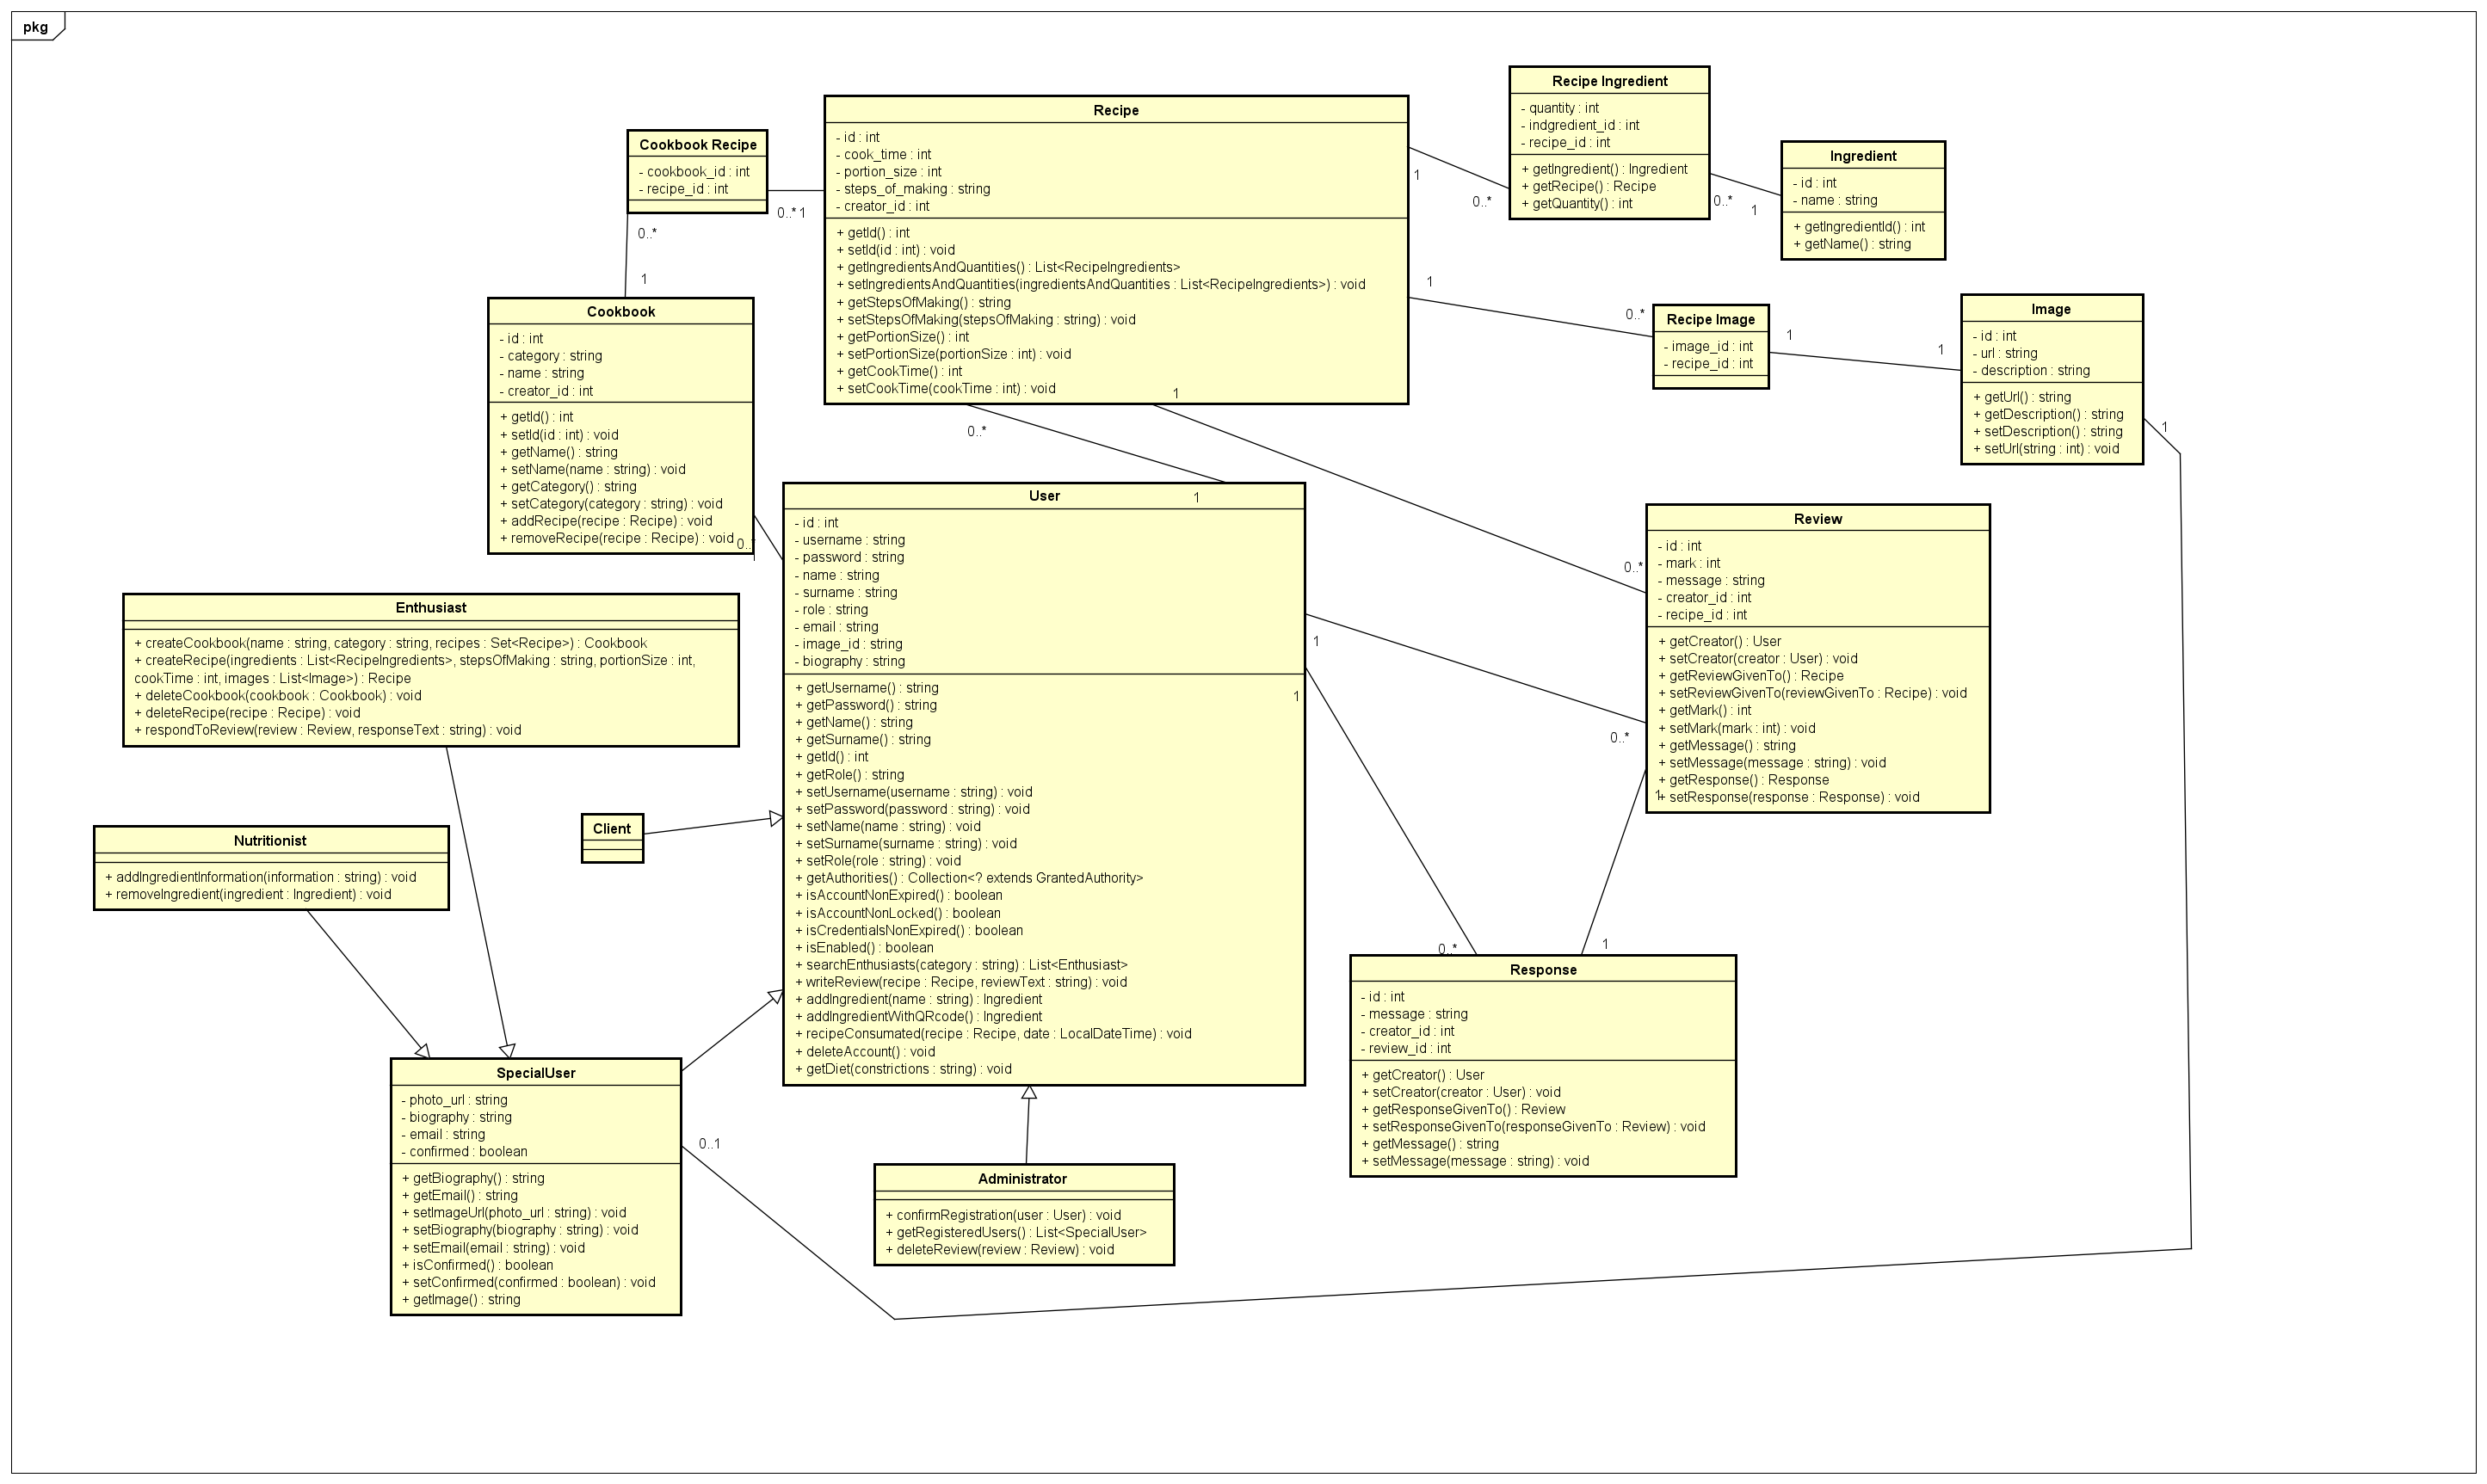
\includegraphics[scale=0.2]{dijagrami/UML_dijagram_razreda_models.png} %veličina slike u odnosu na originalnu datoteku i pozicija slike
			\centering
			\caption{Dijagram razreda - dio Models}
			\label{Dijagram razreda - dio Models}
		\end{figure}
		
Dijagram razreda na slici 4.8 prikazuje \textit{Data Transfer Object} dio razreda. \\
DTO su objekti koji prenose podatke između sustava. Konkretno, kada dođe do zahtjeva za podacima od korisnika na frontendu, DTO razredi koriste se za prijenos tih podataka iz backenda na frontend, koji se zatim prikazuju korisniku koji je poslao zahtjev za njima.

			\begin{figure}[H]
			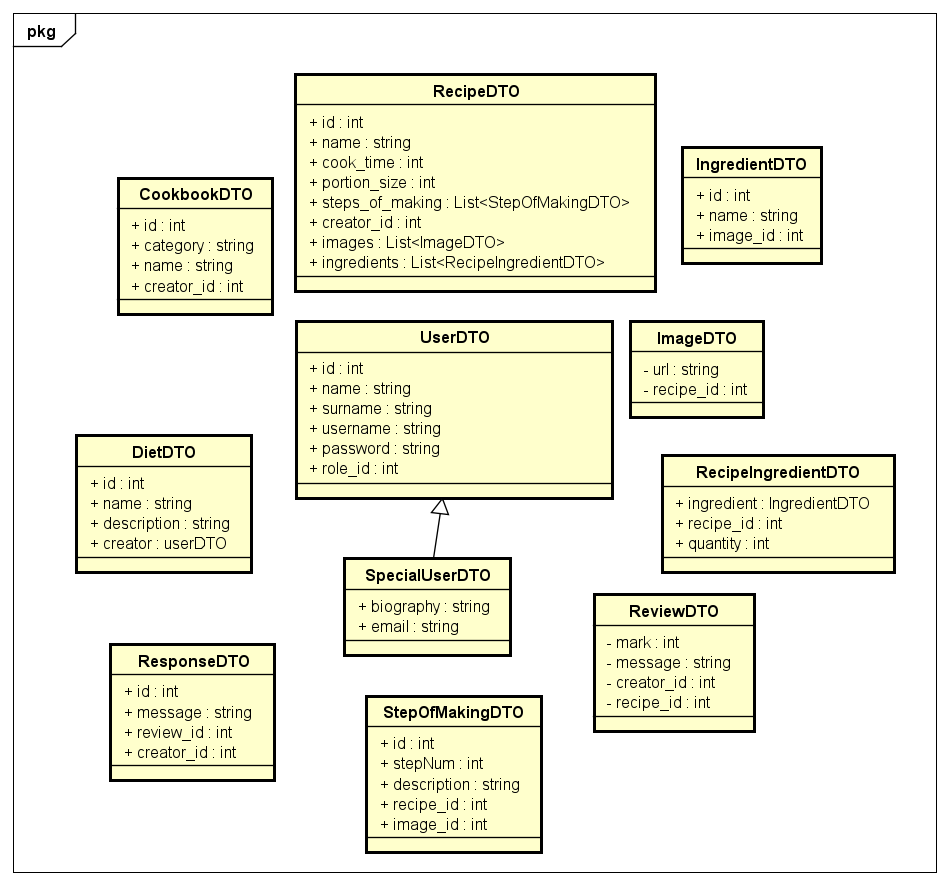
\includegraphics[scale=0.2]{dijagrami/UML_dijagram_razreda_dtos.png} %veličina slike u odnosu na originalnu datoteku i pozicija slike
			\centering
			\caption{Dijagram razreda - dio DTO}
			\label{Dijagram razreda - dio DTO}
		\end{figure}
		
Dijagram razreda na slici 4.9 prikazuje \textit{Repository} dio razreda. \\
Sučelje \textit{Repository} u Spring Boot-u sadrži deklaracije metoda za osnovne operacije vezane uz pristup podacima (čitanje, pisanje, ažuriranje i brisanje).


			\begin{figure}[H]
			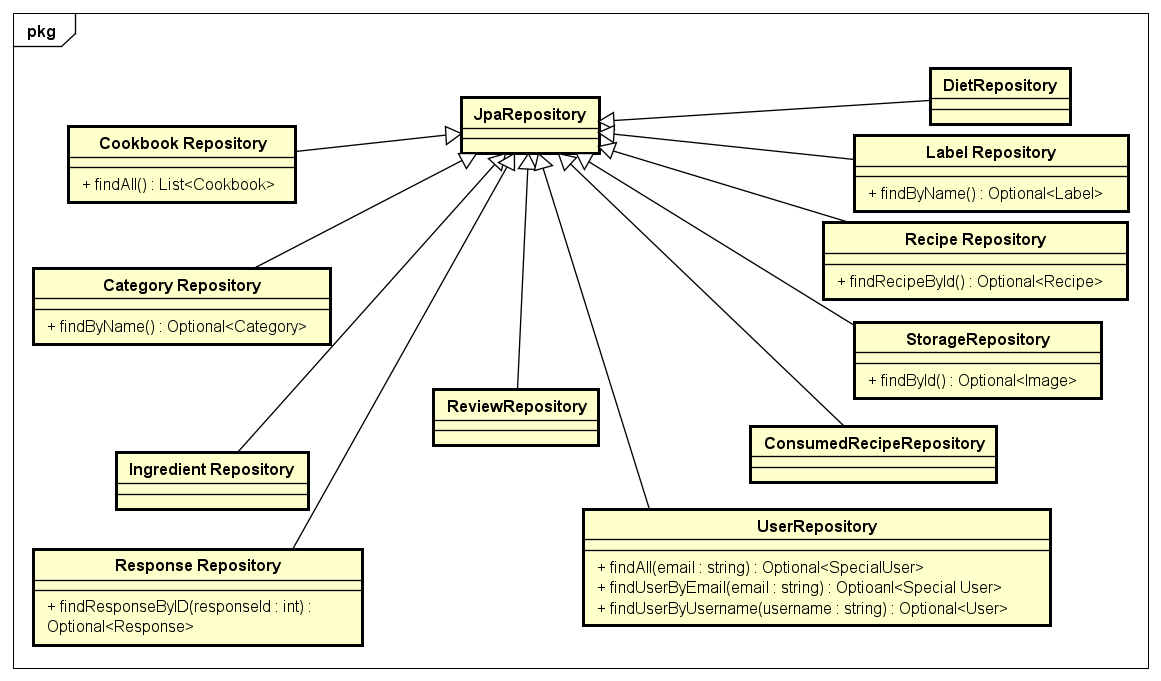
\includegraphics[scale=0.2]{dijagrami/UML_dijagram_razreda_repositories.png} %veličina slike u odnosu na originalnu datoteku i pozicija slike
			\centering
			\caption{Dijagram razreda - dio Repository}
			\label{Dijagram razreda - dio Repository}
		\end{figure} 

Dijagram razreda na slici 4.10 prikazuje \textit{Service} dio razreda. \\
Sučelje servisa definira metode koje su dostupne ostatku aplikacije za izvršavanje implementiranih funkcionalnosti. Često komunicira s metodama iz sučelja \textit{Repository} za pristup podacima, umjesto da izravno komunicira s bazom.


			\begin{figure}[H]
			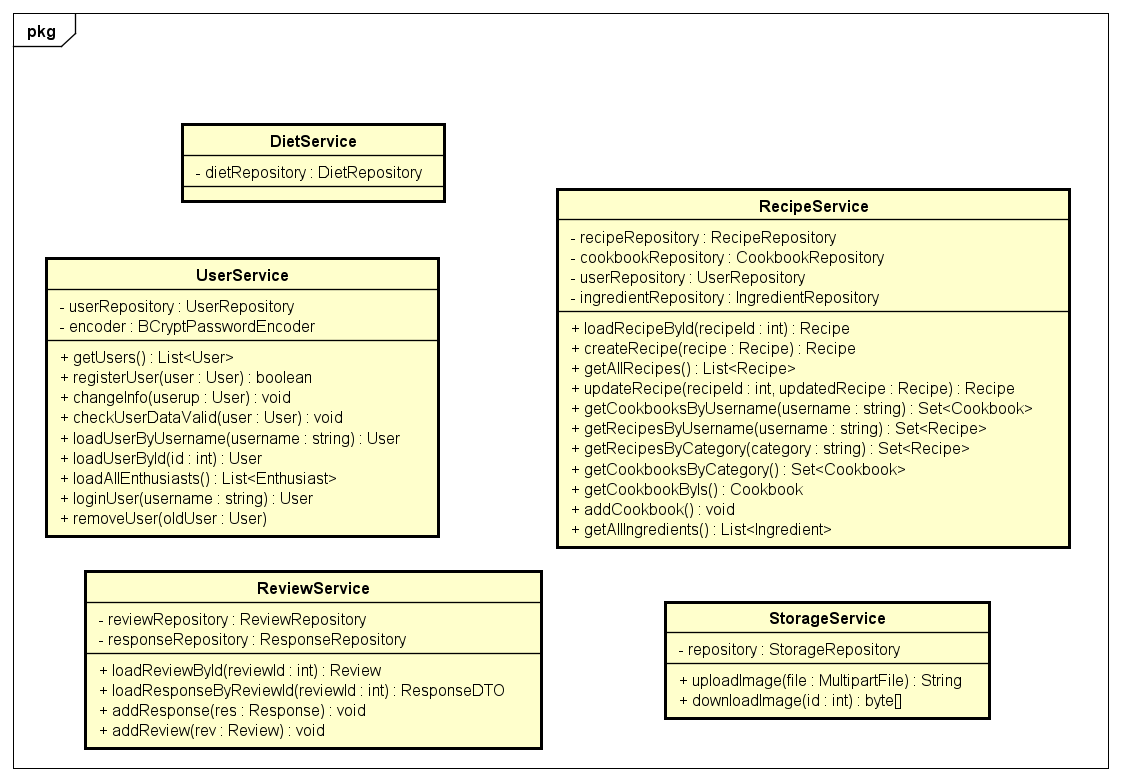
\includegraphics[scale=0.2]{dijagrami/UML_dijagram_razreda_services.png} %veličina slike u odnosu na originalnu datoteku i pozicija slike
			\centering
			\caption{Dijagram razreda - dio Service}
			\label{Dijagram razreda - dio Service}
		\end{figure} 


		\eject
		
		
		\section{Dijagram stanja}
		
		Na slici 4.9 prikazan je dijagram stanja aplikacije implementirane aplikacije KuhajIT. Dijagram stanja je dijagram kojim se prikazuje diskretno ponašanje objekta ili sustava putem prelazaka izmedu konačnog broja stanja. Koristi se za modeliranje ponašanja entiteta tijekom vremena, naglašavajući odgovor na događaje i okidače.
		
		Mi smo odlučili prikazati dijagram stanja za kulinarskog entuzijasta, pošto on ima najviše funkcionalnosti koje su zajedničke svim registriranim korisnicima (klijentima).
		
  Prijavljenom korisniku se na početnoj stranici prikazuju isprobani recepti, informacije o dijeti koju prate, nove kuharice i recepti od drugih kulinarskih entuzijasta koje prate. Također im se nudi sljedeće opcije:
  \begin{itemize}
			\item prikazivanje osobnih podataka
			\item dodavanje nove kuharice
			\item dodavanje novog recepta 
			\item pretraživanje ostalih kulinarskih entuzijasta
			\item odabir recepta / skeniranje QR koda proizvoda
			\item odjava
		\end{itemize}
		
Pri prikazivanju osobnih podataka, klijentu se nudi opcija uređivanja istih. 
Pri dodavanju nove kuharice, kulinarski entuzijast može odabrati želi li odmah dodati i recept u nju, i ako želi, odabrati hoće li to biti neki od njegovih već objavljenih recepata ili želi stvoriti novi recept.
Pri dodavanju novog recepta, kulinarski entuzijast ima priliku odabrati želi li recept dodati nekoj od svojih postojećih kuharica.
Pri dodavanju novog proizvoda, klijent može odabrati želi li skenirati bar kod proizvoda ili ga želi ručno unijeti.

Opcije odjave i prikaza osobnih podataka su svakom prijavljenom korisniku omogućene u bilo kojem trenutku korištenja aplikacije.

			\begin{figure}[H]
			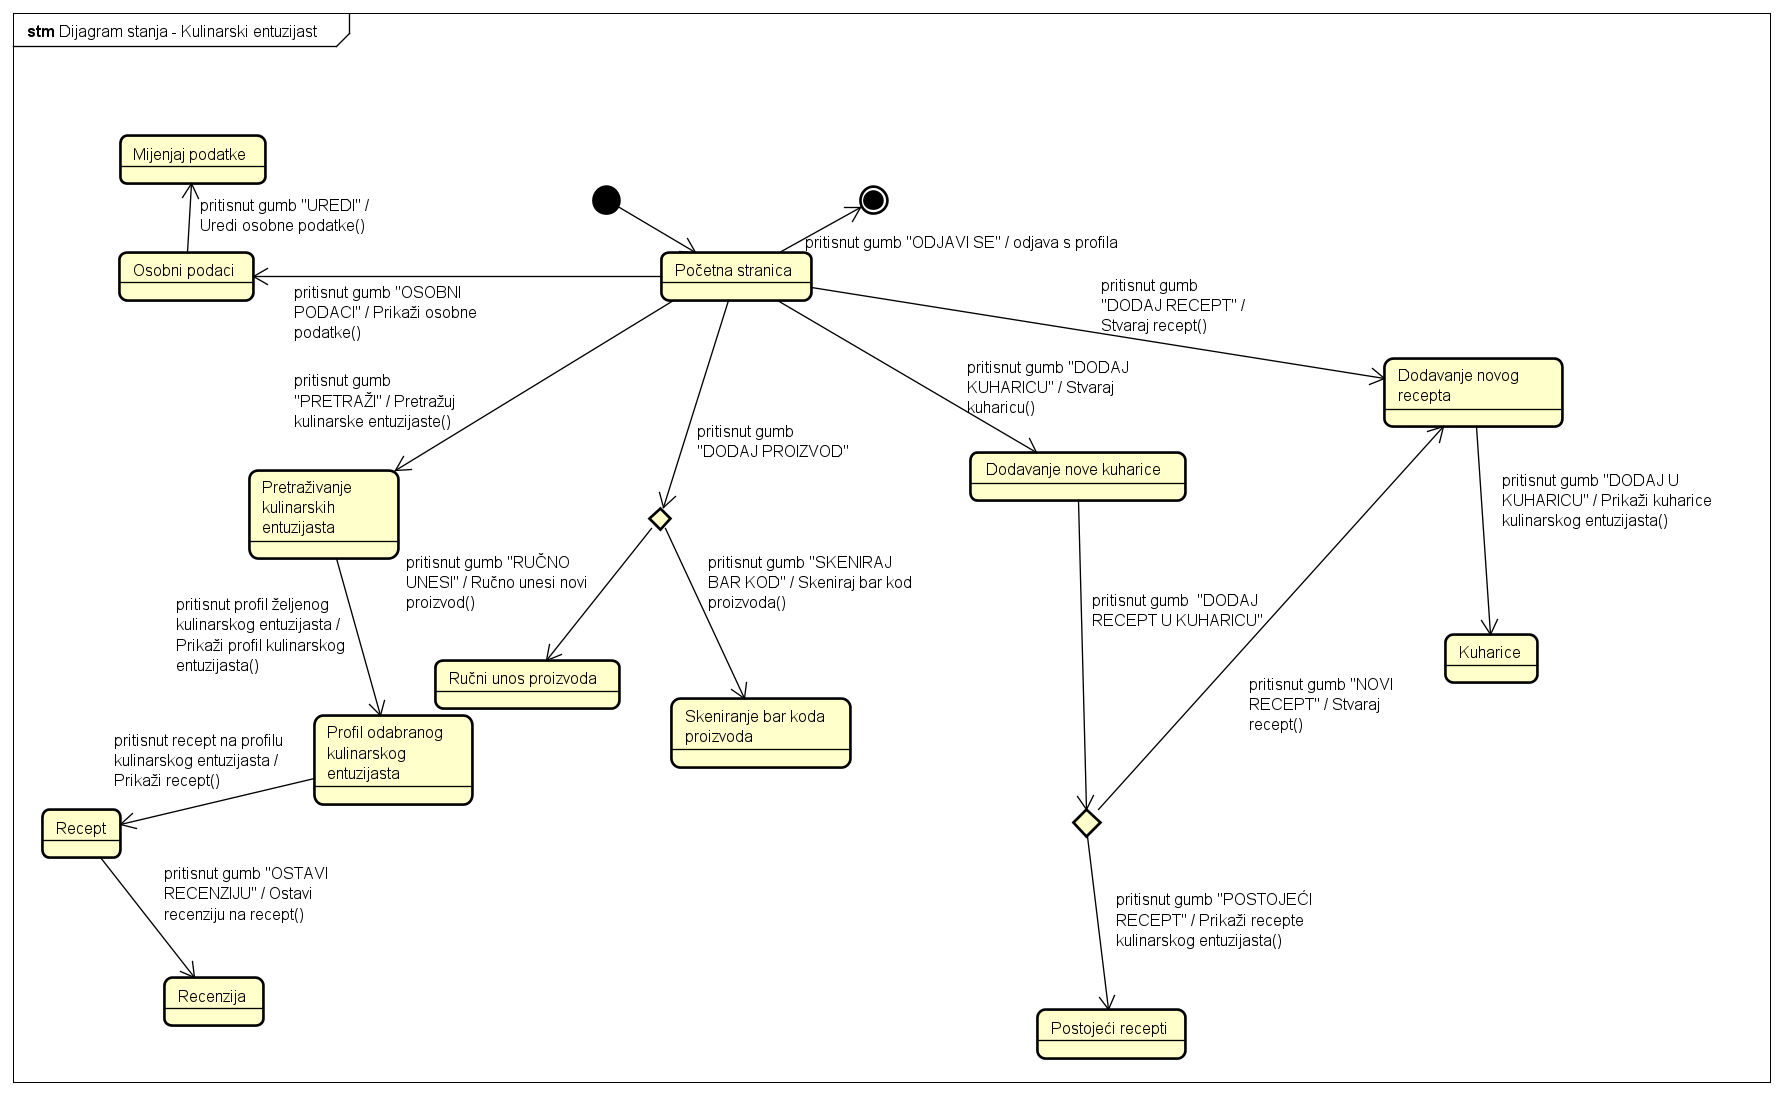
\includegraphics[scale=0.2]{dijagrami/UML_dijagram_stanja.png} %veličina slike u odnosu na originalnu datoteku i pozicija slike
			\centering
			\caption{Dijagram stanja - Kulinarski entuzijast}
			\label{Dijagram stanja - Kulinarski entuzijast}
		\end{figure}
		
		\eject
		
		\section{Dijagram aktivnosti}
		Na slici 4.10 prikazan je dijagram aktivnosti aplikacije KuhajIT. Dijagrami aktivnosti upotrebljavaju se za modeliranje i grafički prikaz dinamičkog ponašanja sustava. Konkretno, na ovom je dijagramu prikazana aktivnost prijave klijenta, unos proizvoda (ručno ili skeniranjem bar koda) te izlistavanje najprikladnijih recepata na temelju unesenih proizvoda i dijete koje se prijavljeni korisnik pridržava.
		
			\begin{figure}[H]
			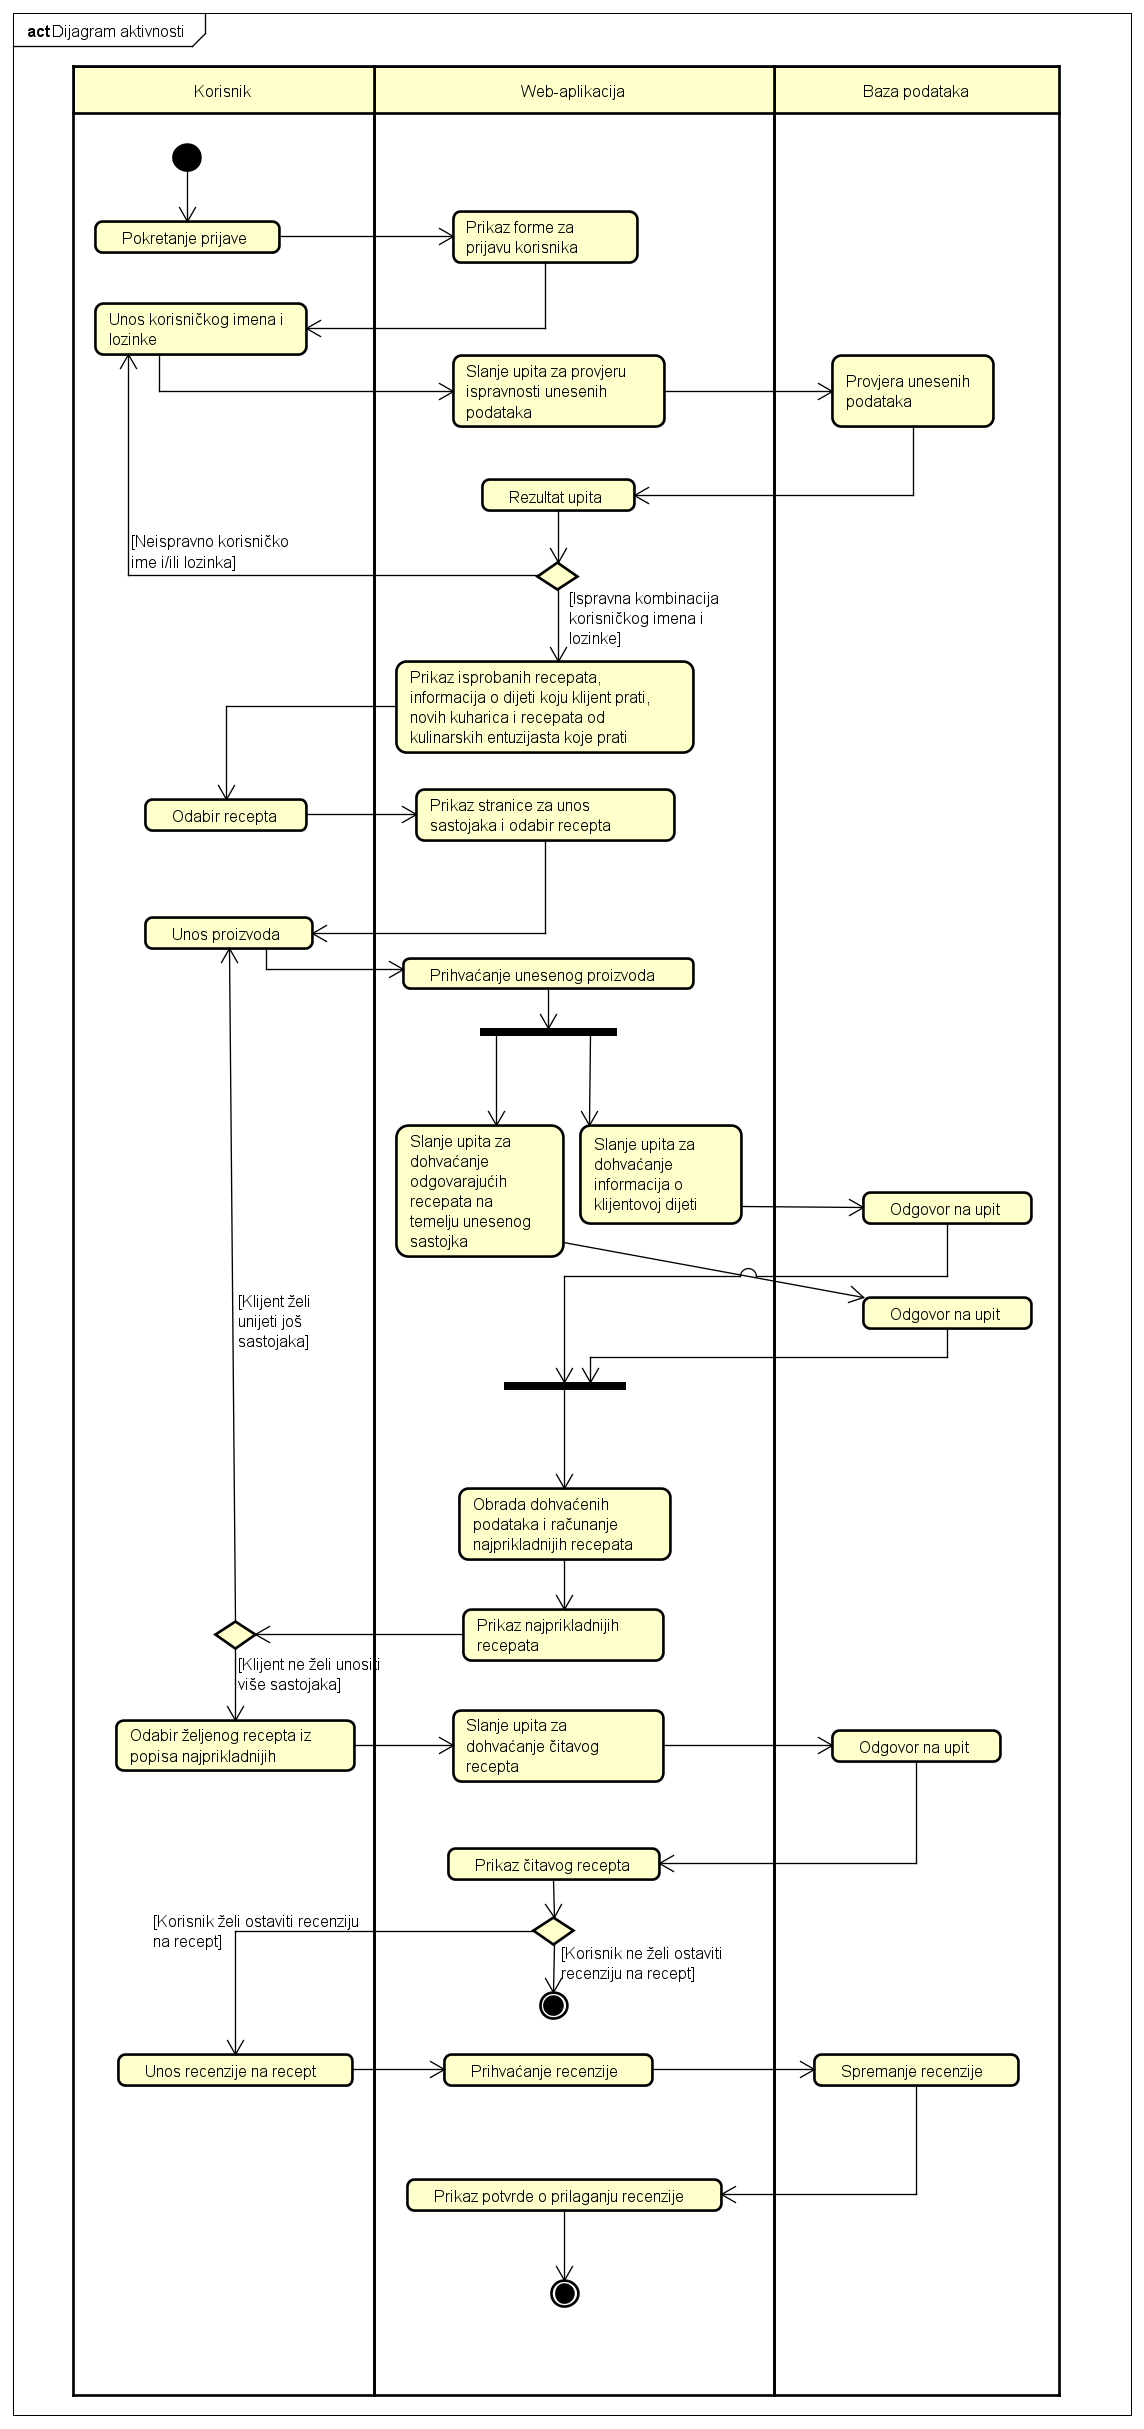
\includegraphics[scale=0.2]{dijagrami/UML_dijagram_aktivnosti.png} %veličina slike u odnosu na originalnu datoteku i pozicija slike
			\centering
			\caption{Dijagram aktivnosti}
			\label{Dijagram aktivnosti}
		\end{figure}
		
		\eject
		
		\section{Dijagram komponenti}
		Na slici 4.11 prikazan je dijagram komponenti. Dijagrami komponenti koriste se za modeliranje arhitekture programskog sustava na visokoj razini. Pružaju jasan i sažet način vizualizacije različitih komponenti ili građevnih blokova sustava i njihovih odnosa.
		
					\begin{figure}[H]
			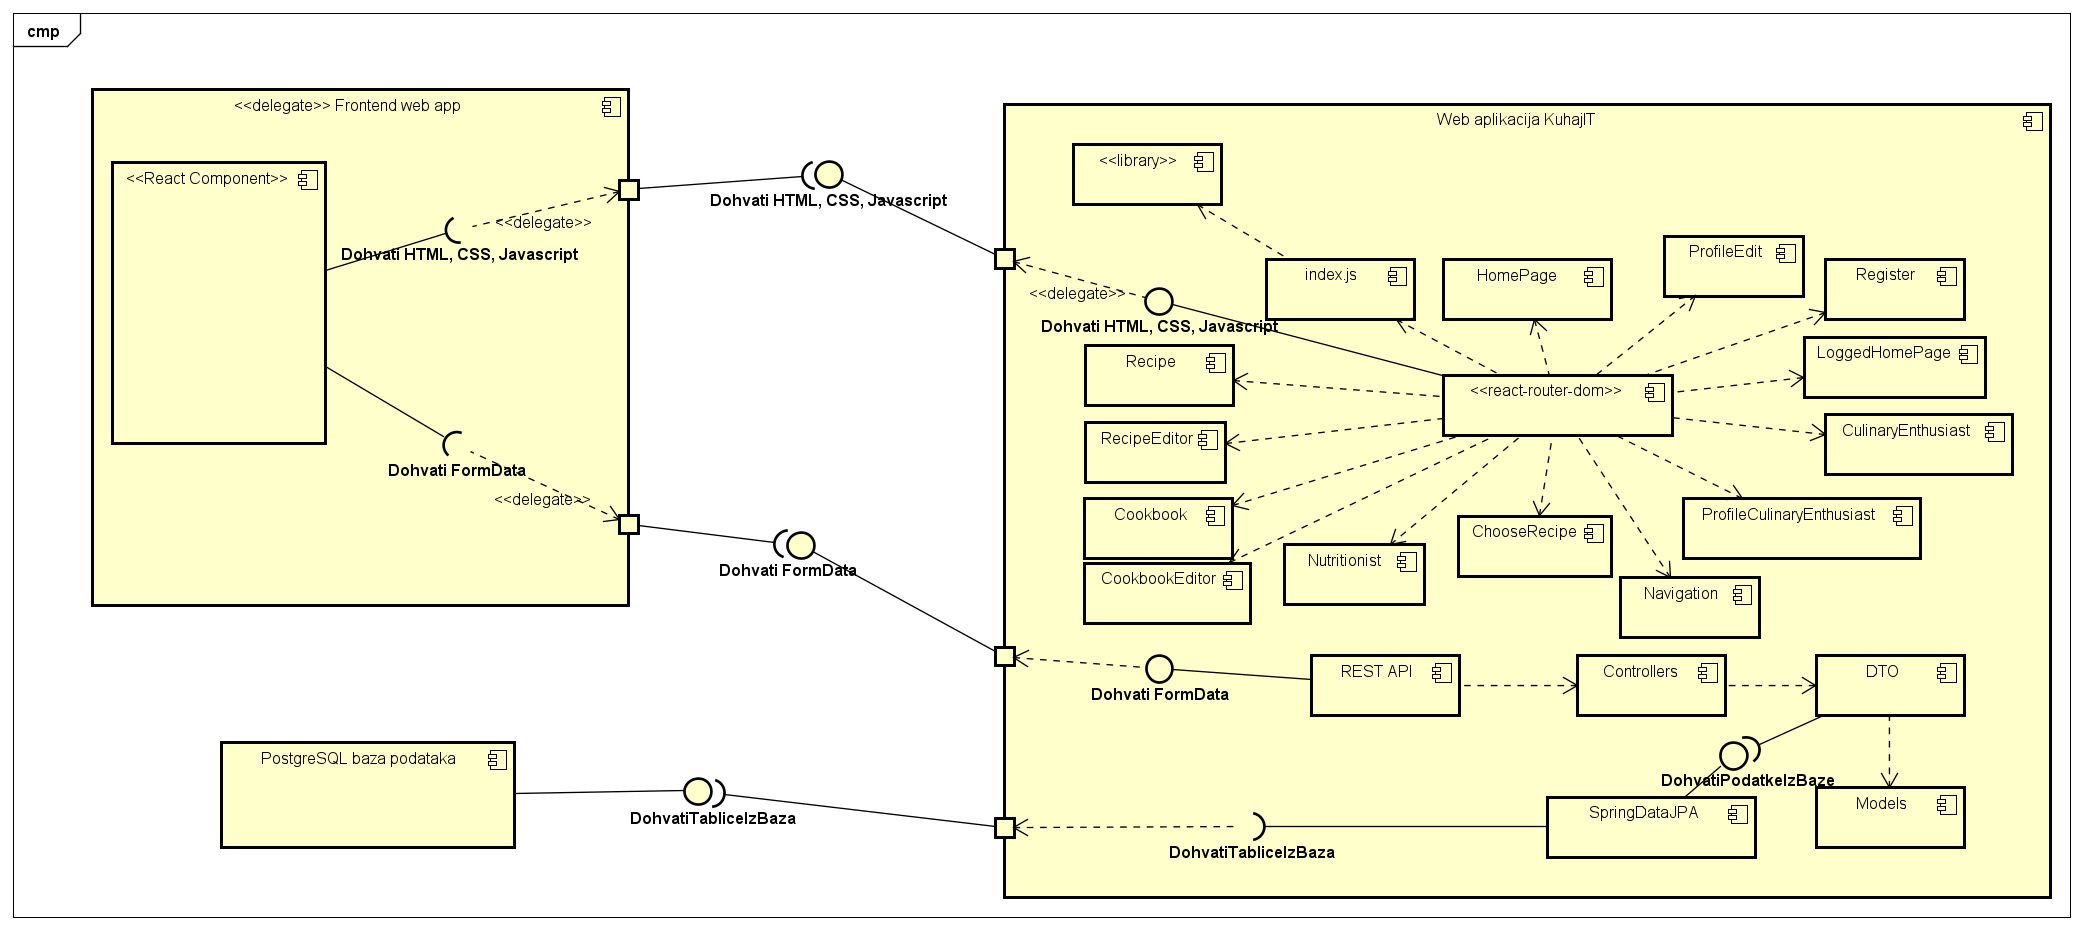
\includegraphics[scale=0.2]{dijagrami/UML_dijagram_komponenti.png} %veličina slike u odnosu na originalnu datoteku i pozicija slike
			\centering
			\caption{Dijagram komponenti}
			\label{Dijagram komponenti}
		\end{figure}
		
		\eject
		
		
		

